\documentclass[a4paper,11pt]{report}
\usepackage[french]{babel}
\usepackage[T1]{fontenc}
\usepackage[utf8]{inputenc}
\usepackage{lmodern}
\usepackage{microtype}
\usepackage{hyperref}
\usepackage{tabulary}
\usepackage{framed}
\usepackage{fancyhdr}
\usepackage{amsmath}
\usepackage{bbm}
\usepackage{graphicx}
\usepackage{pst-all}
\usepackage{xcolor}

%\usepackage{nopageno}

\newcommand{\latin}[1]{\textit{#1}}

\pagestyle{empty}

\pagestyle{fancy}
\fancyhead{}
\renewcommand{\headrulewidth}{0.5pt}
\fancyhead[R]{\textit{\nouppercase{\rightmark}}}
\fancyfoot{}
\renewcommand{\footrulewidth}{0.5pt}
\fancyfoot[L]{\textit{\nouppercase{\leftmark}}}
\fancyfoot[R]{\thepage}
  
\begin{document}
	\begin{titlepage}
		\vspace*{\stretch{2}}
		\begin{center}
			\large\bfseries\itshape Stage ETE 2015\\
		\end{center}
		\noindent\rule{\linewidth}{3pt}

		\begin{center}
			\Huge\bfseries\itshape Description du système\\
		\end{center}
		
		\noindent\rule{\linewidth}{3pt}
		\begin{center}
			\bfseries
			\large F-PHT \\
			\large Un système d'index de filtres de Bloom pour la recherche d'information par mots clés
		\end{center}
		\vspace*{\stretch{2}}
		\begin{center}
			Réalisé par \textbf{DOAN} Cao Sang \\
			Encadrant: M. \textbf{MAKPANGOU} Mesaac, Regal
		\end{center}
		\vspace*{\stretch{0.5}}
		\begin{center}
			1 Juillet 2015
		\end{center}
	\end{titlepage}

\tableofcontents

\chapter{Vue globale}
\section{Prefix Hash Tree (PHT)}
	Un arbre préfixe est un arbre numérique ordonné qui est utilisé pour stocker une table associative où les clés sont généralement des chaînes de caractères. Contrairement à un arbre binaire de recherche, aucun nœud dans le trie ne stocke la chaîne à laquelle il est associé. C'est la position du nœud dans l'arbre qui détermine la chaîne correspondante\footnote{Wikipédia}.
	
	Pour tout nœud, ses descendants ont en commun le même préfixe. La racine est associée à la chaîne vide. Des valeurs ne sont pas attribuées à chaque nœud, mais uniquement aux feuilles et à certains nœuds internes se trouvant à une position qui désigne l'intégralité d'une chaîne correspondant à une clé.
	
	Pour faire une recherche d'une valeur associée à une clé, au départ, on se situe à la racine de l'arbre, en prenant le premier élément de la clé de la requête, on trouve le chemin étiqueté par cet élément, s'il n'existe pas, on est sûr que cette clé n'est pas dans l'arbre. Dès que l'on trouve le chemin, on arrive sur le bon nœud et continue en prenant le deuxième élément de la clé de requête, on applique cette méthode jusqu'à quand on trouve cette clé et se termine sur une feuille.
	
	\begin{figure}[!htbp]
	\centering
	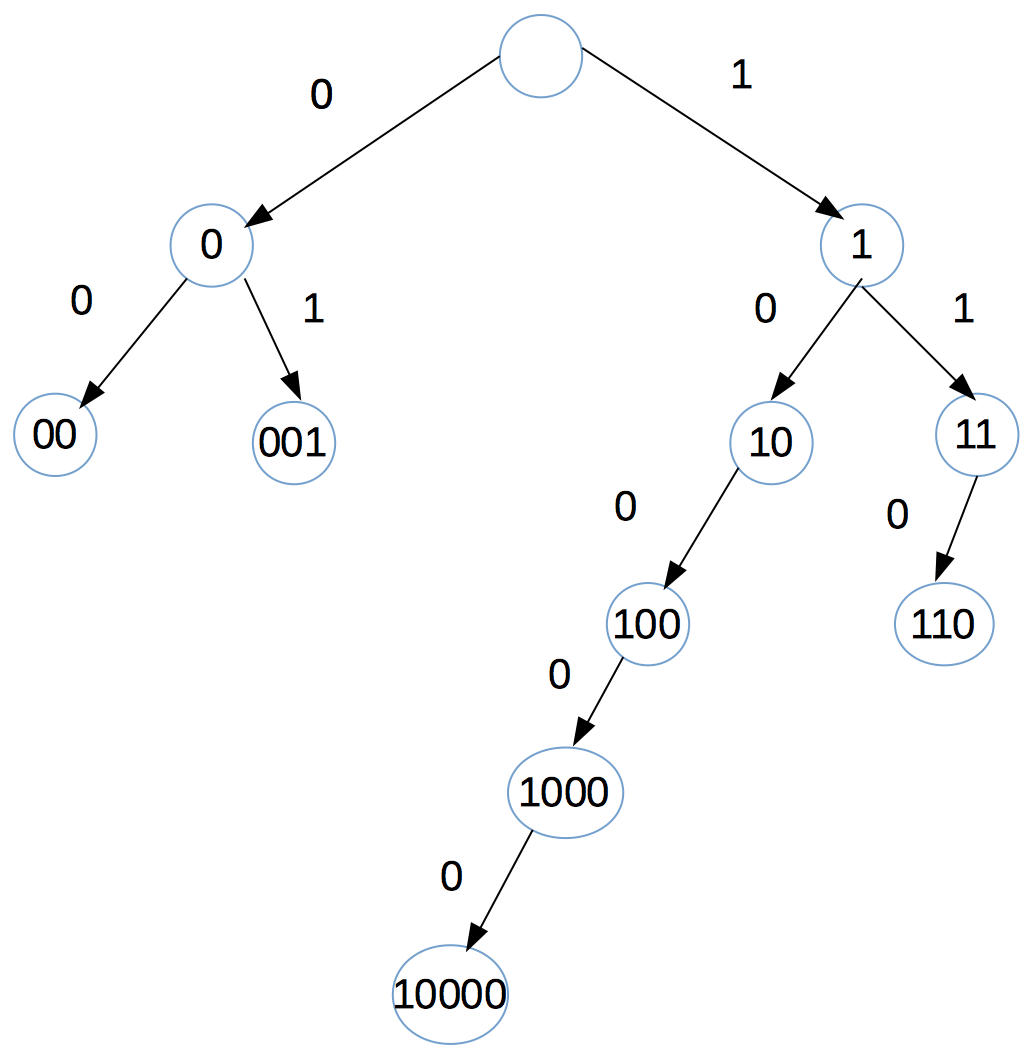
\includegraphics[width=12cm]{PHT.eps}
	\caption{Un arbre de préfixe}
\end{figure}	

\newpage

\section{Fragment}
	On considère un filtre de Bloom de taille \textit{m}. Le système découpe ce filtre en \textit{f} fragments de taille identique. Par convention, les fragments sont numérotés de \textit{0} à \textit{f-1}, en commençant par le fragment le plus à gauche. L'identifiant de chaque fragment est défini de façon unique.
	
		Par exemple, un filtre de Bloom de taille \textit{m = 16} bits, il s'est découpé en \textit{f = 4} fragments, donc chaque fragment est de taille $a = \frac{m}{f} = 4$ bits.

	\begin{table}[!h]
		\centering		
		\begin{tabular}{|l|*{14}{c|}r|}
		\multicolumn{1}{c}{{\scriptsize 15}} &\multicolumn{1}{c}{}&\multicolumn{1}{c}{}&\multicolumn{1}{c}{}&
		\multicolumn{1}{c}{}&\multicolumn{1}{c}{}&\multicolumn{1}{c}{}&\multicolumn{1}{c}{}&
		\multicolumn{1}{c}{}&\multicolumn{1}{c}{}&\multicolumn{1}{c}{}&\multicolumn{1}{c}{}&
		\multicolumn{1}{c}{}&\multicolumn{1}{c}{}&\multicolumn{1}{c}{}&\multicolumn{1}{c}{{\scriptsize 0}}\\
		\hline
			1 & 0 & 0 & \multicolumn{1}{c||}{0} & 
			1 & 1 & 0 & \multicolumn{1}{c||}{1} & 
			0 & 0 & 0 & \multicolumn{1}{c||}{0} & 
			1 & 0 & 1 & 0 \\
		\hline
		\end{tabular}
		\caption{Exemple le filtre de Bloom}
		\label{fragment/filtredeBloom}
	\end{table}

	\begin{table}[!h]
		\centering		
		\begin{tabular}{|l|*{2}{c|}r|}
		\hline
			1 & 0 & 0 & 0 \\
		\hline
		\end{tabular}
		\caption{Exemple la valeur de fragment \textit{0}}
		\label{fragement/exemple1}
	\end{table}

	\begin{table}[!h]
		\centering
		\begin{tabular}{|l|c|c|r|}
		\multicolumn{1}{c}{}&\multicolumn{1}{c}{}&\multicolumn{1}{c}{}\\
		\hline
			1 & 0 & 1 & 0 \\
		\hline
		\end{tabular}
		\caption{Exemple la valeur de fragment \textit{3}}
		\label{fragement/exemple2}
	\end{table}
	
\section{F-PHT}
	F-PHT est une sorte d'arbre préfixe, il utilise  les filtres de Bloom  de taille \textit{m} comme clés de stockage. Cet arbre utilise l'identifiant d'un fragment de filtre de Bloom à la place de préfixe. Chaque nœud de l'arbre stocke un ensemble de couple \textbf{<prefix, identifiant>} avec \textbf{préfix} est la valeur d'un fragment de rang \textit{i} et \textbf{identifiant} est soit l'identifiant d'un nœud, soit \textit{null}. Si \textbf{identifiant} est égal à \textit{null}, \textbf{prefix} est un filtre de Bloom. Sinon, ce couple désigne où sont stockés les filtres de Bloom ayant \textbf{prefix} comme valeur du fragment de rang \textbf{i}, où \textit{i} correspond au niveau de ce nœud dans l'arbre.

	Chaque nœud de rang \textbf{i} contient une table \textbf{RouteEntry}, qui contient les couples stockés par ce nœud. Chaque nœud stocke au plus $\gamma$ couples, avec $\gamma$ inférieur ou égal à $2^{\frac{m}{f}}$. 0 l'initialisation du système, cette table est vide, elle sont remplit au fur et à mesure automatiquement. Une fois, la capacité a été débordée, le système éclate ce nœud en créant des nouveaux fils de rang \textit{i+1} et met à jour la table \textbf{RouteEntry}.
	
\section{Système d'indexation}
	Le système d'indexation est un système qui indexe les données pour faciliter la recherche de données, il gère en général une très grande quantité de données. Dans le cadre de mon travail, ce système arrange les données dans un arbre F-PHT en utilisant le filtre de Bloom pour générer les clés de stockage et aussi les données.
	
	Ce système dispose les actions comme:
	\begin{itemize}
		\item Ajout d'un filtre de Bloom dans le système.
		\item Cherche d'un filtre de Bloom.
		\item Suppression d'un filtre de Bloom.
	\end{itemize}
	
\subsection{Ajout d'un filtre de Bloom dans F-PHT}
	Comme le F-PHT utilise des fragments d'un filtre de Bloom comme clés de stockage, le système crée un fragment \textit{$R_i$} de niveau \textit{i}, au départ \textit{i = 0} comme le rang de la racine. Ensuite, à partir de ce fragment, un couple \textit{<$R_i$,null>} est soumit à la racine pour ajout dans l'arbre. La façon de traitement dans chaque nœud dépend la nature de ce nœud, un nœud ou une feuille.

\subsubsection{Cas d'un nœud feuille de rang i dans F-PHT}
	Tant que la capacité de la table \textbf{RouteEntry} qui stocke les couples terminaux dans ce nœud feuille est inférieure à $\gamma$, chaque nouveau couple terminal qui arrive sur ce nœud feuille est simplement ajouté dans \textbf{RouteEntry}.

	Une fois, la capacité de cette table atteint, elle ne peut plus stocker des nouveaux couples qui arrivent. Donc, dans ce cas, le nœud feuille exécute une opération interne du système d'indexation pour qu'elle puisse les ajouter. \textbf{split()} est une opération utilisée lors que le système veut éclater un nœud, les étapes sont:
	\begin{enumerate}
		\item 
	\end{enumerate}
\subsubsection{Cas d'un nœud de rang i dans F-PHT}
	
	

\end{document}









